\chapter{Memorie a stato solido} 

Abbiamo già visto come è  fatta una memoria RAM, alle bitline si attaccano due inverter messi in feedback, con dei pass transistor accediamo al contenuto il quale verrà letto grazie al sense amplifier. 

\section{Memorie ROM}

Tutto questo per una cella ROM, memoria non scrivibile, tutto questo processo  è più semplice. Per far si che in una cella venga memorizzato un bit (0,1) non è necessario che si inserisca un Flip-Flop o un condensatore come nella RAM dinamica, l'importante che la bitline vada a 0 oppure 1 quando si seleziona la cella corrispondente.

\paragraph{}
Dunque è un po' come la DRAM, attacchiamo al transistor da una parte la bitline e dall'altra a massa al posto del condensatore. Il transistore porta a zero il contenuto quindi la bitline leggerà zero, per leggere invece un uno dobbiamo proprio togliere il transistore! 


\begin{figure}[htbp]
    \centering
    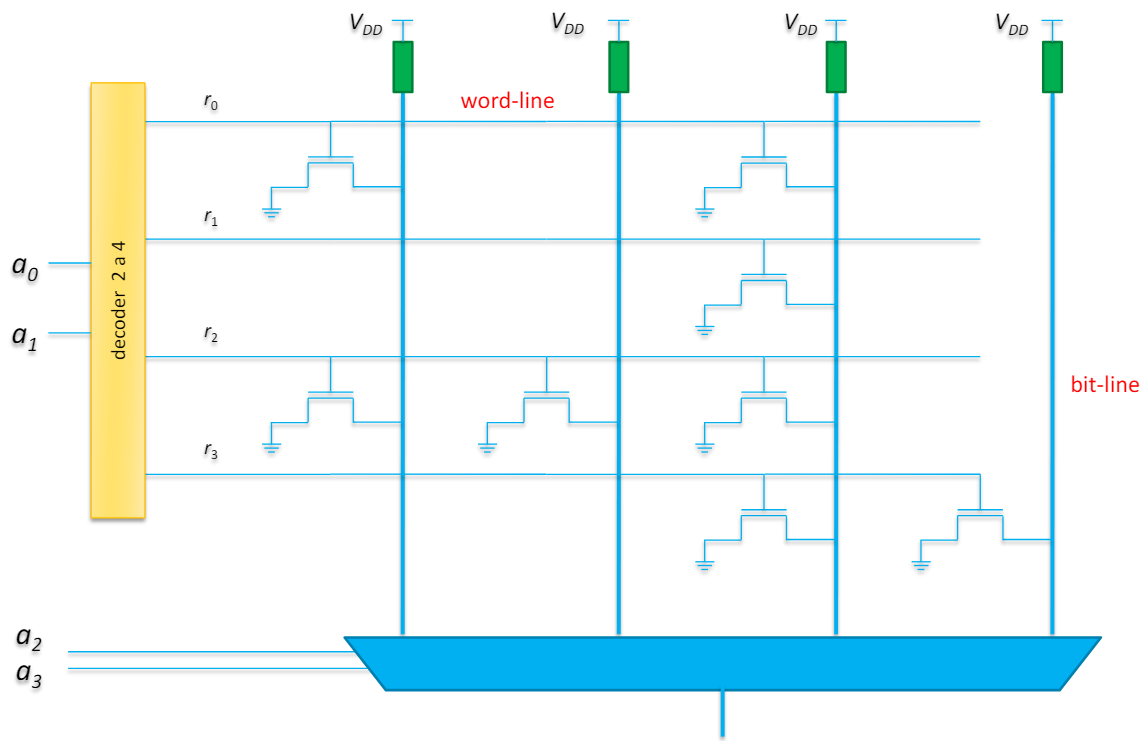
\includegraphics[width=0.7\linewidth]{img/mhtjg.png}
    \caption{16-bit ROM}
\end{figure}

\paragraph{NOTA:} la bitline viene caricata prima con il valore 1. Inoltre questa è una memoria costruita così infatti non è programmabile ma è di sola lettura.

\newpage
\section{Memorie Flash - riscrivibili e non volatili}
La memoria Flash è non volatile e riscrivibile. A differenza della memoria DRAM,
prima di potere procedere alla scrittura devono essere cancellati dei blocchi di dati,
con conseguente riduzione delle prestazioni di scrittura rispetto a quelle di lettura.
La memoria Flash supporta solo un determinato numero di operazioni di scrittura, che
varia a seconda della tecnologia utilizzata.

\paragraph{}
La memoria Flash è disponibile come NAND o NOR. I prodotti SSD utilizzano la memoria
Flash NAND perché garantisce una durata maggiore, è meno costosa, le celle sono più
dense e le operazioni di cancellazione/scrittura sono più veloci rispetto alla memoria
Flash NOR. 

La memoria Flash NOR viene utilizzata per memorizzare il codice binario
di programmi in quanto è caratterizzata da prestazioni molto elevate in lettura.

\subsection{Il Floating gate transistor}

Per rendere la cella di memoria riscrivibile si utilizza un particolare transistor chiamato \textbf{Floating gate transistor}.


\begin{figure}[htbp]
    \centering
    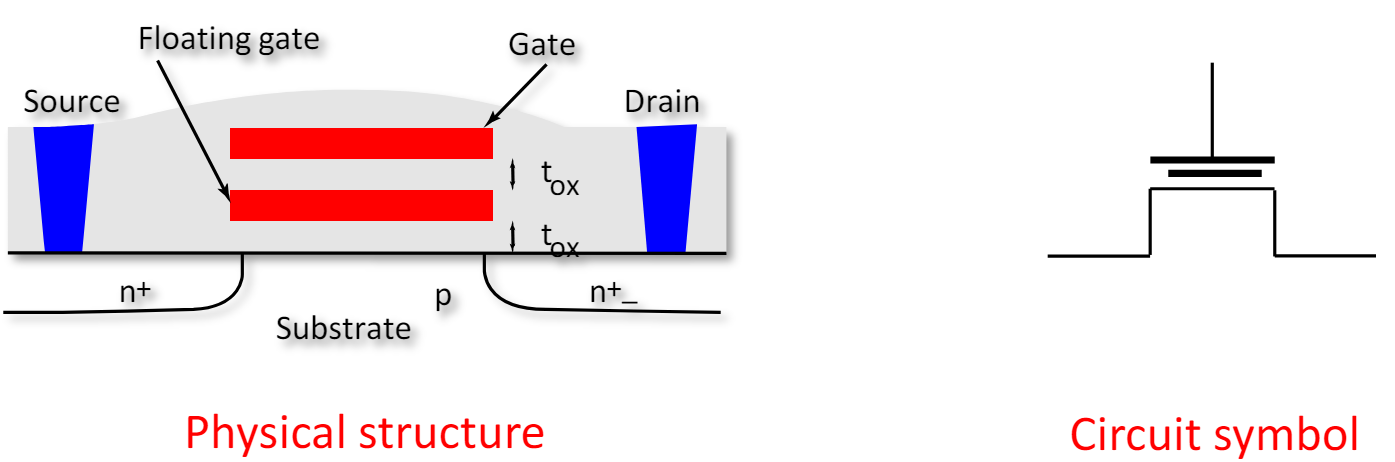
\includegraphics[width=0.5\linewidth]{img/mhgytf.png}
    \caption{Floating gate transistor}
\end{figure}

La particolarità è che ha due gate, il più in altro è quello standard, quello più vicino al gate è \textbf{isolato} e \textbf{flottante}, il quale viene interposto tra il gate ed il canale. 

A parte l’incremento dello spessore dell'ossido, il floating gate altera anche la tensione di soglia e dunque possiamo cambiarla a piacimento, vediamo come.

\subsection{Programmazione}

\begin{figure}[htbp]
    \centering
    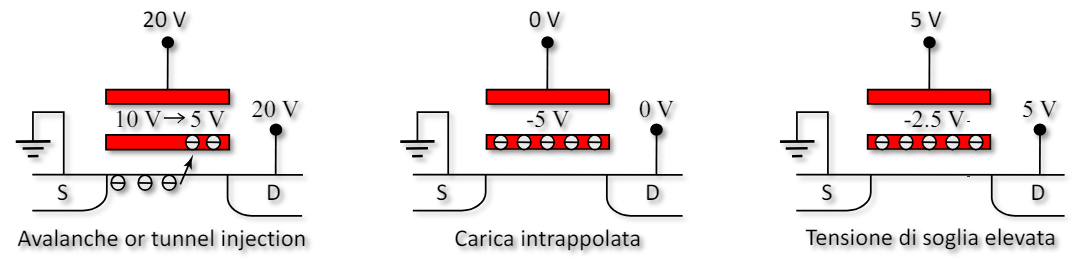
\includegraphics[width=0.7\linewidth]{img/hmg.png}
\end{figure}

Vogliamo mettere, spostare, delle cariche su questo flottante, inizialmente il metallo è neutro, ha tanti protoni quanti elettroni. Per far in modo di depositarvi sopra delle cariche si deve aumentare di molto la tensione di alimentazione posta sul gate.

 Il campo elettrico attira gli elettroni nel canale verso l'isolante, se questa energia è abbastanza elevata questi elettroni passano attraverso l'ossido di silicio per \textbf{effetto valanga} (alta energia), si deve dare tanta tensione al drain,  o per \textbf{effetto tunnel}, fenomeno della meccanica quantistica che si verifica quando lo strato di ossido è particolarmente sottile e applicando una grande tensione al gate le cariche si spostano,  arrivando nel gate di mezzo.

 \paragraph{}
 Caricato il gate di mezzo con degli elettroni, le quali cariche bilanciano già le cariche sul gate, ora il gate per formare il canale per mettere in comunicazione il drain e il source, la tensione di gate deve essere ancora più alta di quella di un transistore normale, senza il floating gate (cariche in più). 
 
 Dunque mettendo delle cariche nel floating gate l'effetto è stato quello di \textbf{alzare la tensione di soglia} del transistore. Questa carica potrebbe permanere anche per diversi anni!

 \paragraph{}
 Il transistor non può più essere portato in conduzione (con le
tensioni normali), ed è come se non ci fosse, circuito aperto.


\section{Memorie EPROM}
Le memorie EPROM, Erasable Programmable Read Only Memory,  funzionano proprio così, sono delle memorie con dei floating gate.


\begin{figure}[htbp]
    \centering
    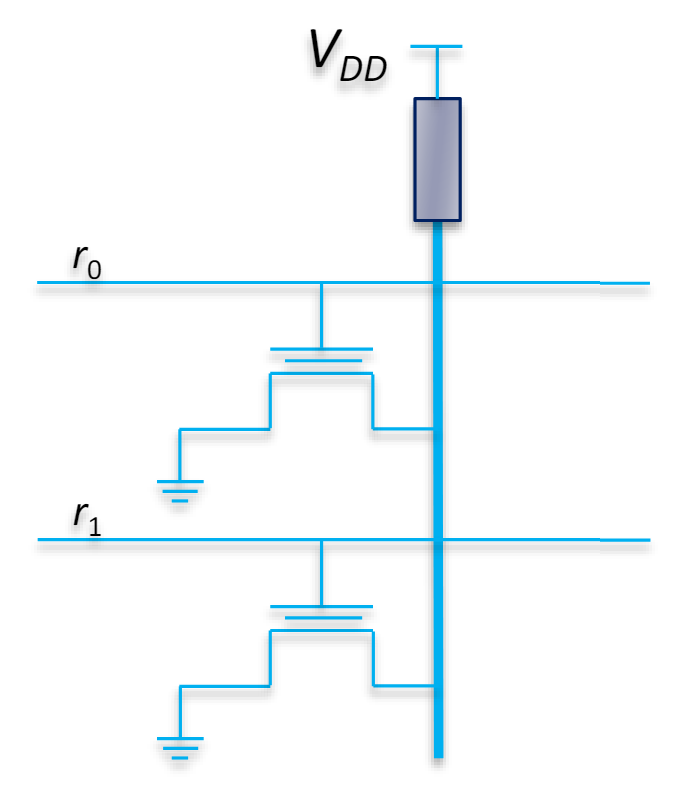
\includegraphics[width=0.27\linewidth]{img/bsf.png}
    \caption{Memorie EPROM}
\end{figure}

Se abbiamo messo le cariche negative sul floating gate, abbiamo programmato un uno, perché la tensione applicata al gate (2.5 V, tensione normale) non è abbastanza per superare la tensione di soglia (si e sempre in \textbf{cut-off}). Se non le avessimo messe, allora c'è uno zero, perché attivando il gate con 2.5 V il canale si forma e la bitline va a massa e legge zero, si comporta come un transistore normale.

\paragraph{}
Come detto prima, essendo il gate flottante, queste cariche non vanno più via. Una volta per eliminare la carica nei circuiti caricati con \textbf{effetto valanga} si lasciava piccola finestrella la quale serve perché una volta irraggiato di raggi UV per numerosi minuti, la carica scendeva attraverso il substrato e il circuito ritornava programmabile. Questo processo però degrada notevolmente il substrato il quale dopo un po' di cicli non regge più e il circuito risulta da buttare.

\paragraph{}

Nei circuiti caricati con \textbf{effetto tunnel}, il processo di rimozione è molto semplice, basta fare il contrario, quindi applicare una tensione molto negativa al gate per far scivolare via le cariche dal floating gate.

Comunemente oggi si utilizzano le \textbf{EEPROM} o \textbf{$E^2\text{PROM}$}: Eletrically Erasable Programmable Read Only Memory, tuttora non sono nemmeno più di sola lettura ma anche di scrittura.

\paragraph{NOTA:} per vedere se il transistore è stato programmato oppure no, al gate basta mettere una tensione che sta tra le due soglie e:

\begin{itemize}
    \item Se non è programmato il transistore si accende;
    \item Se è programmato non si accende.
\end{itemize}




\begin{figure}[htbp]
    \centering
    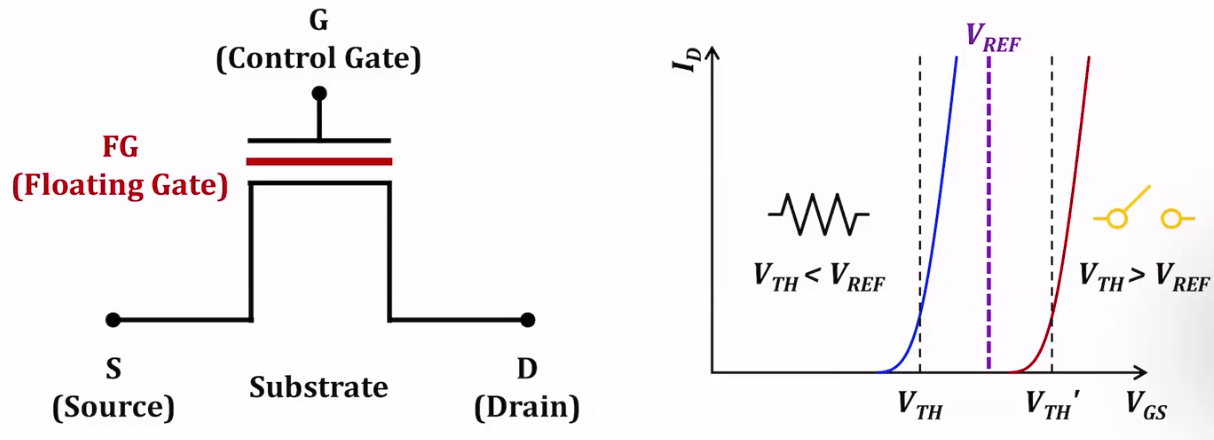
\includegraphics[width=0.6\linewidth]{img/dnfg.png}
\end{figure}

\newpage
\section{SSD basate su memoria Flash NAND}

Nelle moderne architetture Flash, si può decidere quanta carica mettere nel floating gate, infatti sono multi livello, ovvero possiamo programmare diversi modelli di logica all'interno del floating gate.

In una cella normale la cella o è carica oppure si possono rappresentare multi livelli, quindi più bit.

\begin{figure}[htbp]
    \centering
    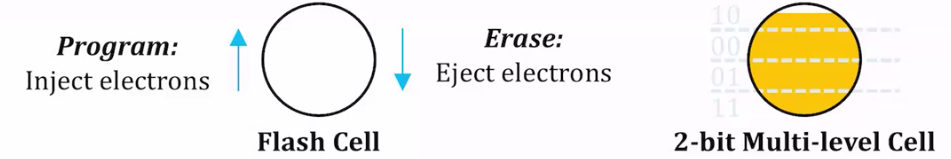
\includegraphics[width=0.55\linewidth]{img/nmfhg.png}
    \caption{Multi-level cell}
\end{figure}

Il problema è che la carica dopo del tempo si perde fino ad arrivare ad avere un errore questo può capitare spesso nelle celle multi livello. Per ovviare a questo le Flash normalmente hanno dei bit aggiuntavi per della ridondanza e correzione. 
\paragraph{}
Oltre a questo man mano che si fanno letture e scritture abbiamo elettroni che passano attraverso il substrato grazie all'effetto tunnel i quali danneggiano quest'ultimo tendendo sempre di più ad essere meno isolante. Nel caso in cui si rilevano errori frequenti, quella cella verrà marchiata come non usabile. Per ovviare a questo problema, il controllore dell'SSD, molto sofisticato, cerca di scrivere un po' ovunque per mantenere una usura quantomeno omogenea.


\begin{figure}[htbp]
    \centering
    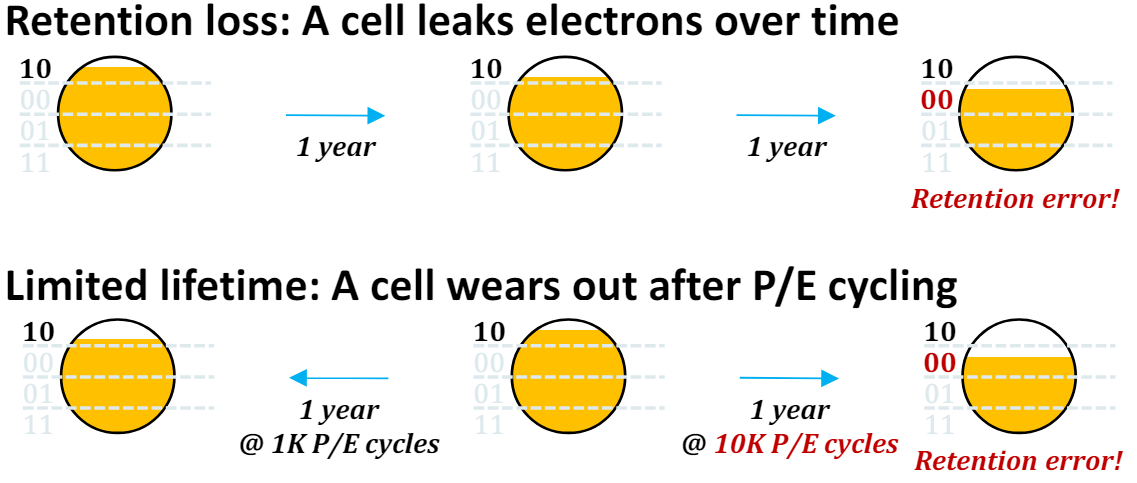
\includegraphics[width=0.55\linewidth]{img/mfhg.png}
\end{figure}

Le celle inoltre diventano più lente in quanto si fa sempre più fatica a discriminare il livello che vi è salvato al suo interno.

\subsection{Organizzazione delle celle}

Prima abbiamo visto che l'organizzazione delle celle, ad esempio la cella di memoria EPROM, era organizzata come una NOR.

\begin{figure}[htbp]
    \centering
    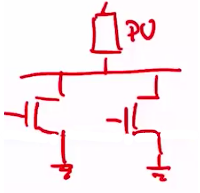
\includegraphics[width=0.2\linewidth]{img/sfbdv.png}
\end{figure}

Questa configurazione è possibile, il problema è che occupano molto spazio, vedremo in seguito il perché.

Quello che invece possiamo fare è quello di organizzare le celle in serie, creando appunto una \textbf{NAND string}.

\newpage

\begin{figure}[htbp]
    \centering
    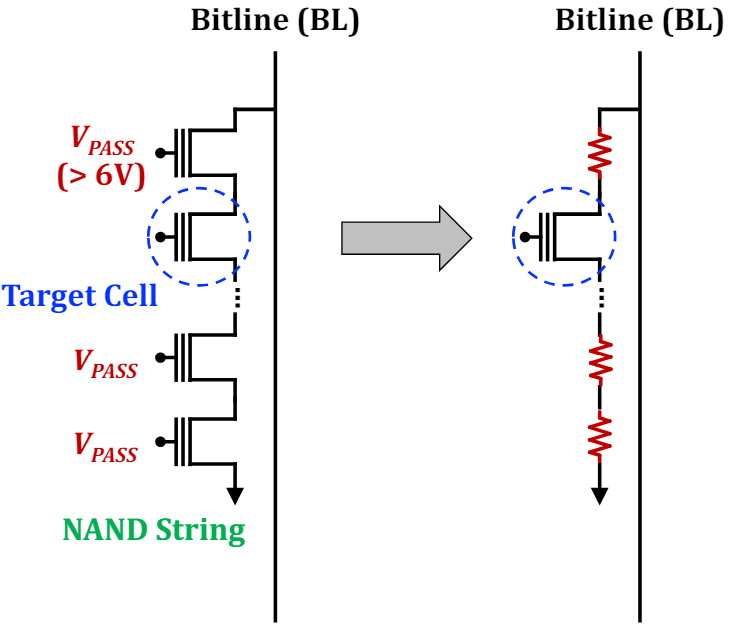
\includegraphics[width=0.5\linewidth]{img/mhgj.png}
    \caption{NAND string}
\end{figure}

Se nella NOR per leggere una cella agli altri ingressi mettiamo zero, nella NAND invece tutti gli ingressi dobbiamo metterli ad uno! Perché si comportino come dei cortocircuiti, dobbiamo mettere una tensione $V_{PASS}$, maggiore della più alta soglia possibile che si può programmare,  sulle celle che non vogliamo leggere, mentre una tensione normale per la cella che vogliamo leggere.

\subsection{NOR vs. NAND layout}

Anche il layout è in favore della NAND, in quanto ha una densità maggiore, questo è dovuto al fatto che non vi è un contatto, la parte N collega un transistore al successivo senza doversi attaccare alla bitline.

\begin{figure}[htbp]
    \centering
    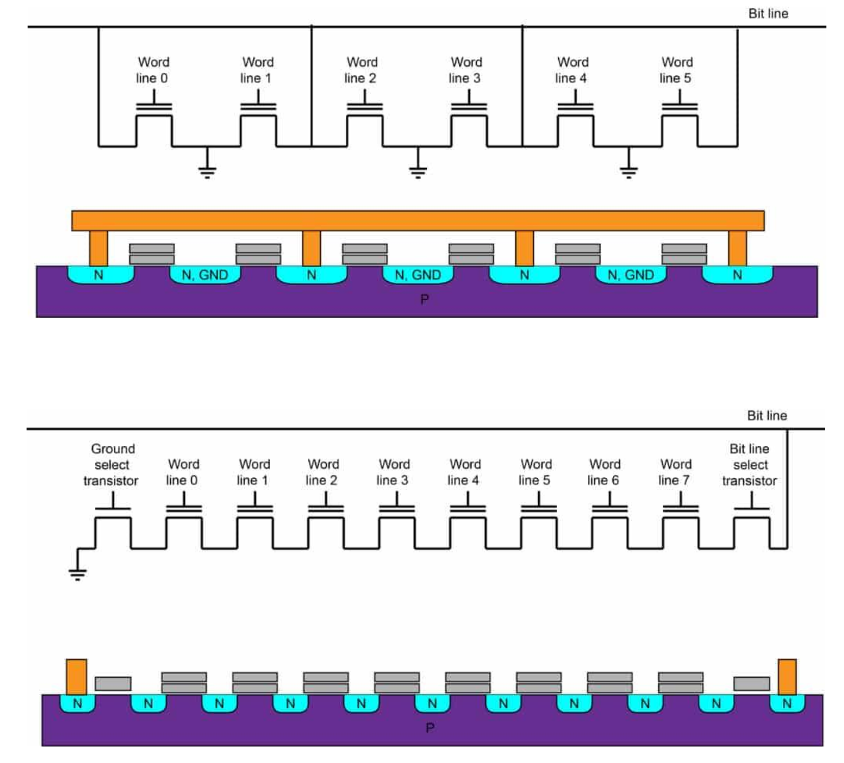
\includegraphics[width=0.5\linewidth]{img/ahnertd.png}
    \caption{NOR vs. NAND layout}
\end{figure}


\newpage

\begin{table}[h!]
\centering
\caption{Confronto tra celle NAND e NOR}
\label{tab:nand_nor}
\begin{tabular}{ c|c|c }

Caratteristica & Celle NAND & Celle NOR \\ \hline
Costo & Più economico & Più costoso \\
Densità & Più densa & Meno densa \\
Prestazioni di scrittura & Più veloci & Più lente \\
Durata & Più lunga & Più corta \\
Accesso casuale & Supportato & Non supportato \\
Esecuzione del codice & Non supportato & Supportato \\
Velocità di lettura & Più lenta & Più veloce \\ 
\end{tabular}
\end{table}

\paragraph{NOTA:} un possibile uso delle memorie Flash NOR è quello di installarci il BIOS dato che si vuole avere una lettura molto veloce anche a scapito della dimensione.


\section{Organizzazione interna memorie NAND - pagine e blocchi}

Nelle moderne architetture le memorie contengono un elevato numero ($>100\,000$) di celle che operano in modo concorrente, sempre organizzate con uno schema a matrice.

\begin{figure}[htbp]
    \centering
    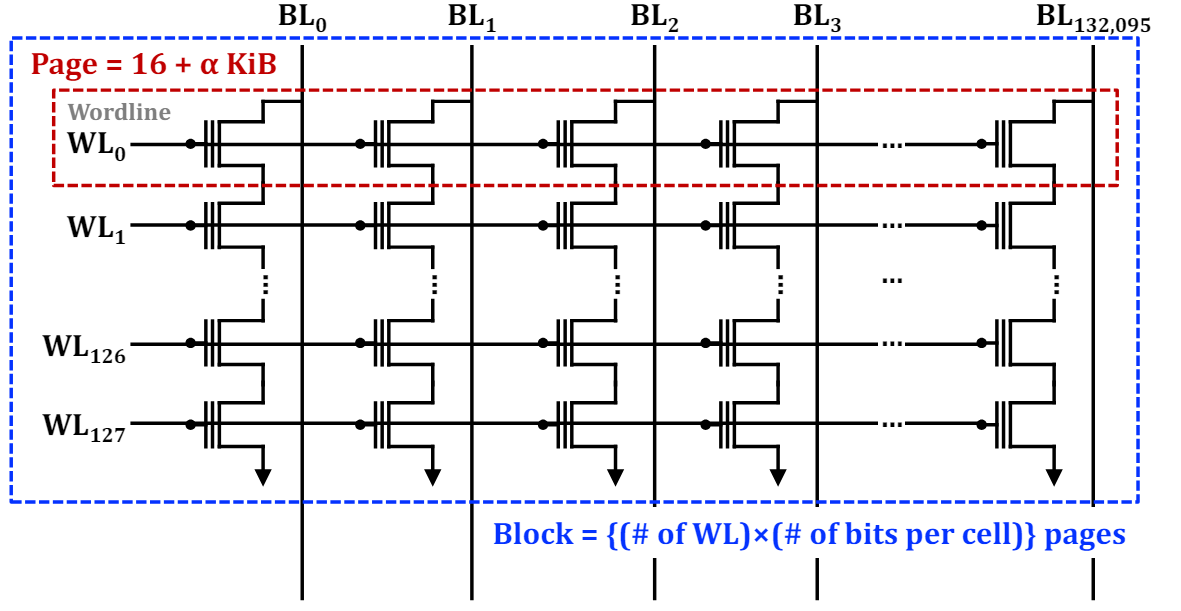
\includegraphics[width=0.65\linewidth]{img/ndg.png}
    \caption{NAND - 128 wordline}
\end{figure}

Possiamo vedere che un blocco contiene molte pagine, in questo caso da $16 + \alpha \,KiB$, dove $\alpha$ è un numero di bit usato per la ridondanza e correzione di errori.

\subsection{Cancellazione e scrittura}
Il processo di cancellazione, decremento della tensione $V_{TH}$, e scrittura, incremento della tensione $V_{TH}$, nella SSD avviene per blocchi, perché la cancellazione è molto lenta essendo che dobbiamo regolare con precisione la quantità di carica che finisce nei transistori. Togliendogli troppa carica si crea un condensatore che starà sempre acceso il quale porterà sempre allo stesso valore la bitline e quella bitline non potrà essere più utilizzata.

\paragraph{}

Questo processo infatti solitamente è iterativo in cui si aggiunge carica a poco a poco e si verifica dove si è arrivati. Ecco perché della scrittura a blocchi, ricordiamo anche che pure nei vecchi dischi magnetici si scriveva a blocchi, infatti il file system pressoché è rimasto invariato.

\paragraph{}
Solitamente dunque quando si deve cambiare dei valori in un blocco, il blocco vecchio lo si elimina piano piano e si scrive il nuovo valore in un'altra parte del disco, così da mantenere anche un usura uniforme. Per cambiare il valore di una cella \textbf{NON è possibile} farlo, proprietà "cancella prima di scrivere".

\newpage
\section{Piani}

Un gran numero di blocchi ($> 1\,000$), uno sopra l'altro, condividono la bitline e anche altri circuiti per la scrittura e lettura, in un \textbf{piano}.

Un possibile elemento condiviso potrebbe essere il \textbf{decoder} il quale selezione il blocco opportuno. Per far si che il blocco venga selezionato si devono aggiungere due pass transistor, i quali verranno entrambi attivati, per far attaccare la stringa alla bitline.

\begin{figure}[htbp]
    \centering
    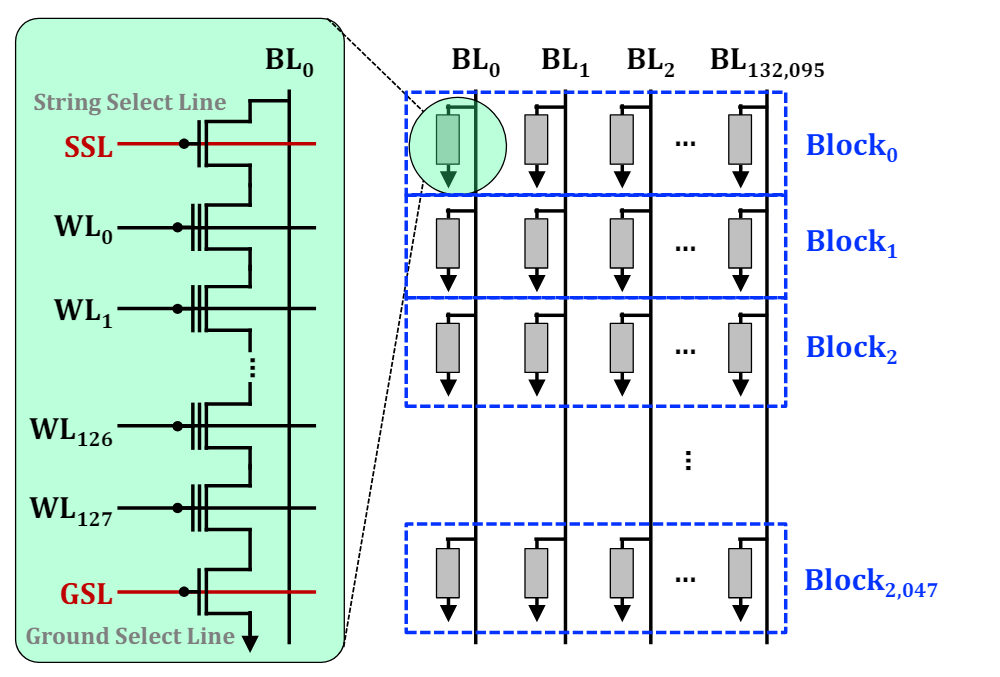
\includegraphics[width=0.65\linewidth]{img/mhg.png}
    \caption{Piano con $2\,048$ righe}
\end{figure}

\section{Dies}

Un Die o un chip contengono molteplici piani (2 - 4).

\begin{figure}[htbp]
    \centering
    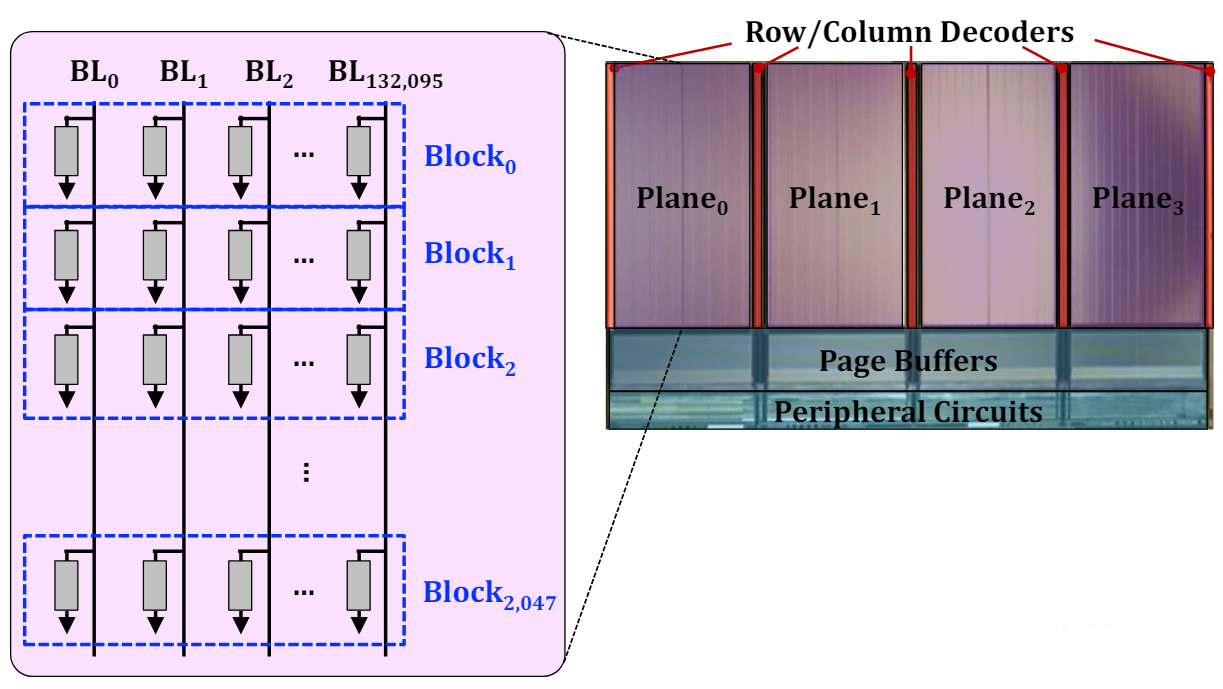
\includegraphics[width=0.65\linewidth]{img/dbsf.png}
    \caption{21-nm 2D NAND Flash Die}
\end{figure}

I piani condividono i decoders dunque vi sono dei limiti interni per il parallelismo, una sola operazione allo stesso instante di tempo, a dire il vero si possono fare delle operazioni in parallelo su piani diversi, però sulla stessa riga, utile per della ridondanza.

\newpage
\section{Distribuzioni dei livelli logici per una memoria NAND}

Ogni transistore non ha un valore specifico per quando il dato è programmato o cancellato, dunque i livelli compressivi di tutti i transistori seguono l'andamento di una gaussiana.

Tra le sue gaussiane vi deve essere abbastanza spazio in mezzo per discriminare, un po' come il margine di rumore, se si incontrassero le due gaussiane non riusciremmo più a distinguere se la cella è programmata o meno.

Tutto questo discorso vale ancora di più se si pensa alle celle multi-bit.

\begin{figure}[htbp]
    \centering
    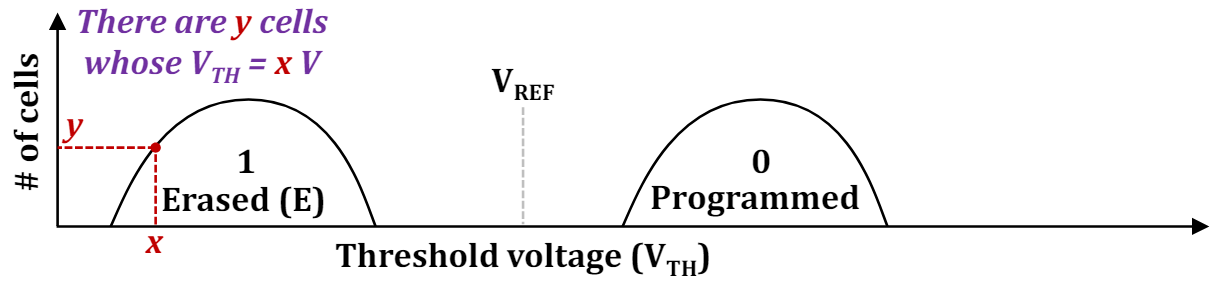
\includegraphics[width=0.65\linewidth]{img/Immagine 2024-05-21 185733.png}
\end{figure}



\subsection{Cella multi bit a 8 livelli}

\begin{figure}[htbp]
    \centering
    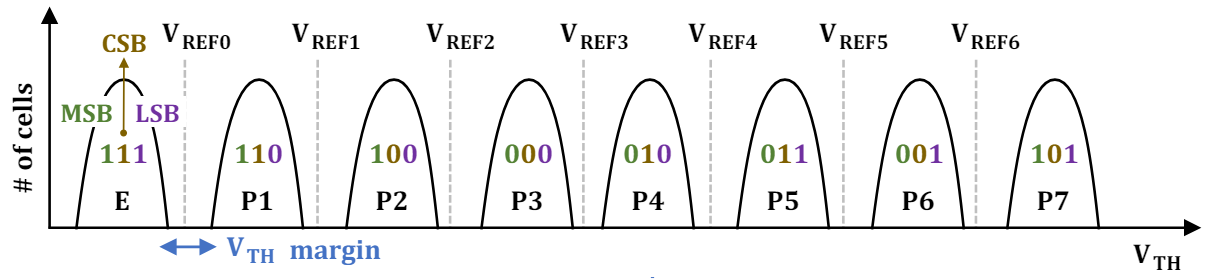
\includegraphics[width=0.65\linewidth]{img/fdsbbfsg.png}
    \caption{Triple Level Cell}
\end{figure}

\section{Programmazione}

Abbiamo detto che la programmazione avviene per pagine intere, quindi innanzitutto si deve mettere il livello di programmazione, $V_{PROG}$, $20\,V$, alla bitline. Tutti gli altri floating gate si deve mettere un livello tale da superare anche la soglia più alta, $V_{PASS}$, $V_{PASS} < V_{PROG}$. I transitori di accesso basta attivarli, $V_{DD}-V_{CC}$.



\begin{figure}[htbp]
    \centering
    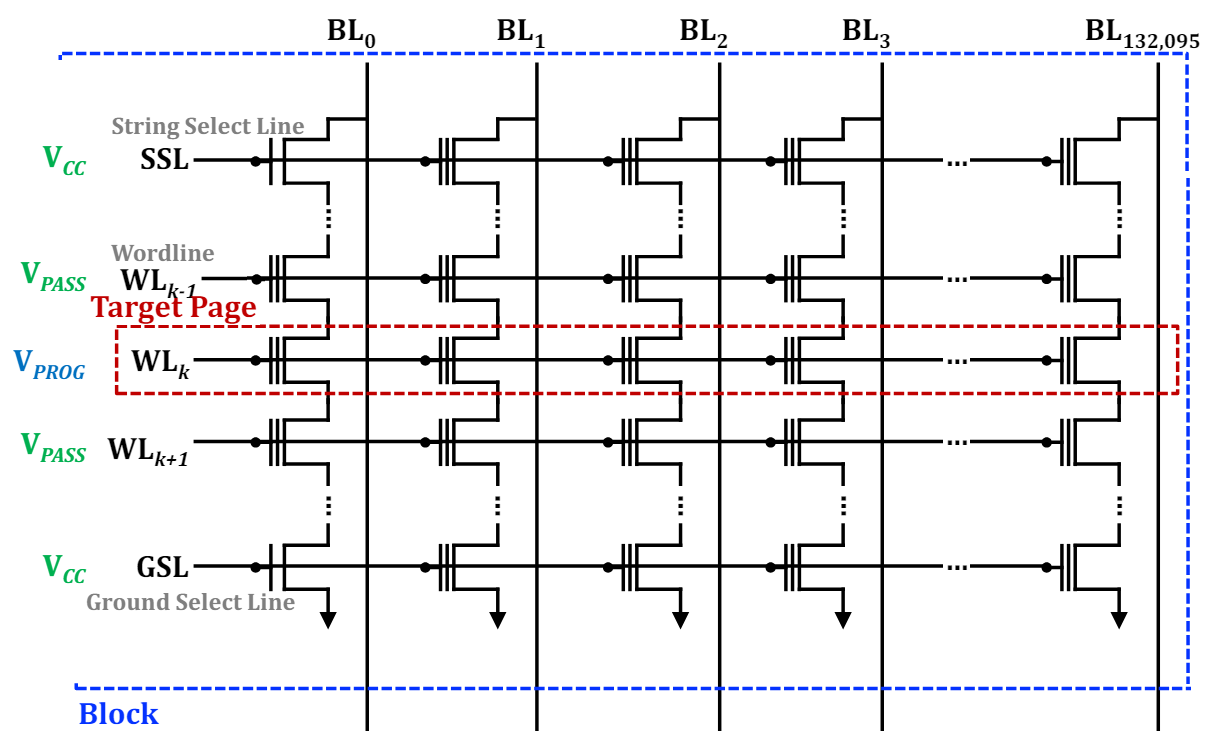
\includegraphics[width=0.65\linewidth]{img/aejmt.png}
\end{figure}


\newpage
Dunque i transistor che non devono essere scritti si comportano come una resistenza, mentre  la pagina verrà tutta programmata. Noi non vogliamo però programmarla tutta con lo stesso valore, bensì con valori diversi: alcuni vogliamo programmarli altri no.


\begin{figure}[htbp]
    \centering
    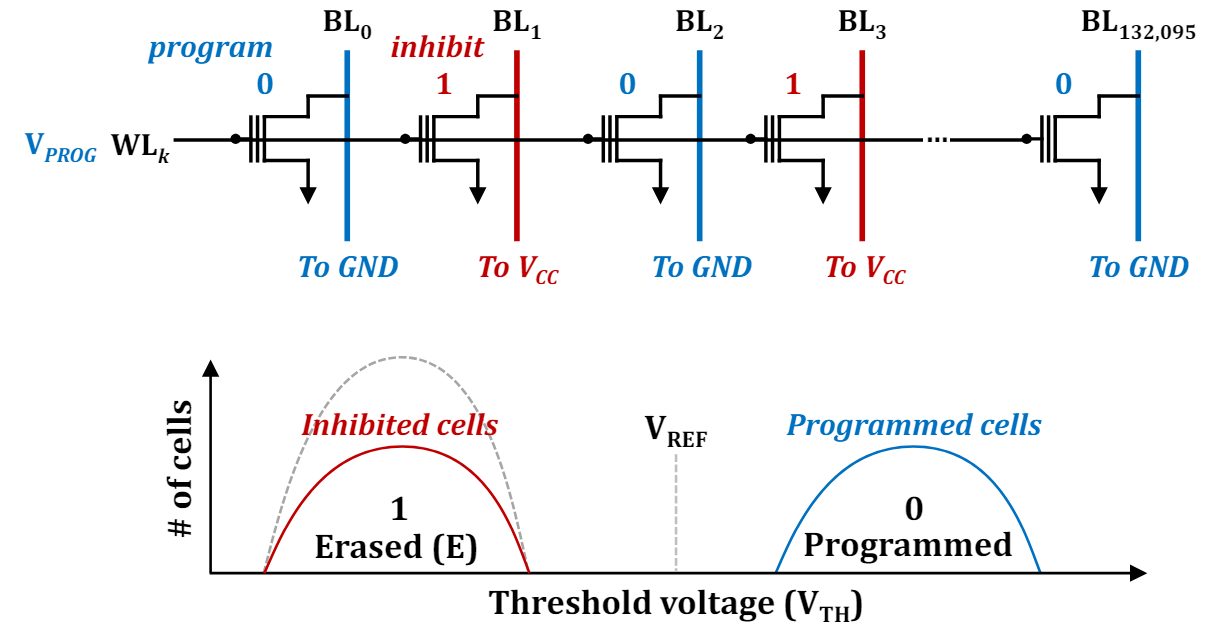
\includegraphics[width=0.7\linewidth]{img/ajryt.png}
\end{figure}

Per programmare basta agire sulla bitline, mettendola a GND tra il gate e il substrato c'è la tensione massima, se non si vuole programmare, basta portare alla stessa tensione del gate pure la bitline facendo si che la differenza di potenziale sia zero e dunque non programmiamo nulla. 

\paragraph{}

Agendo sulle bitline possiamo decidere che valore vogliamo dentro ogni singola cella di tutta la pagina selezionata con la wordline.

\section{Lettura}

Ora non mettiamo più la tensione di programmazione, $V_{PROG}$, bensì la tensione che sta a metà, $V_{PROG}$. Quindi sopra la soglia normale $V_{T}$ ma sotto $V_{PROG}$. Le bitline possiamo metterle alla tensione di alimentazione $V_{CC}$ e andare a vedere su quale stringa sta passando corrente, altrimenti si possono precaricare e si può vedere quelle che si scaricano.

\begin{figure}[htbp]
    \centering
    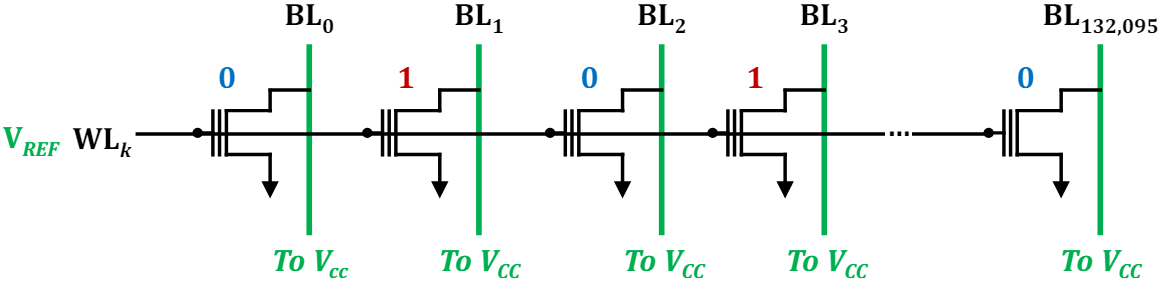
\includegraphics[width=0.6\linewidth]{img/andfg.png}
\end{figure}

Qualunque metodo utilizziamo, riusciamo a leggere un intera pagina. Se passa corrente significa che il valore è uno, viceversa zero.


\begin{figure}[htbp]
    \centering
    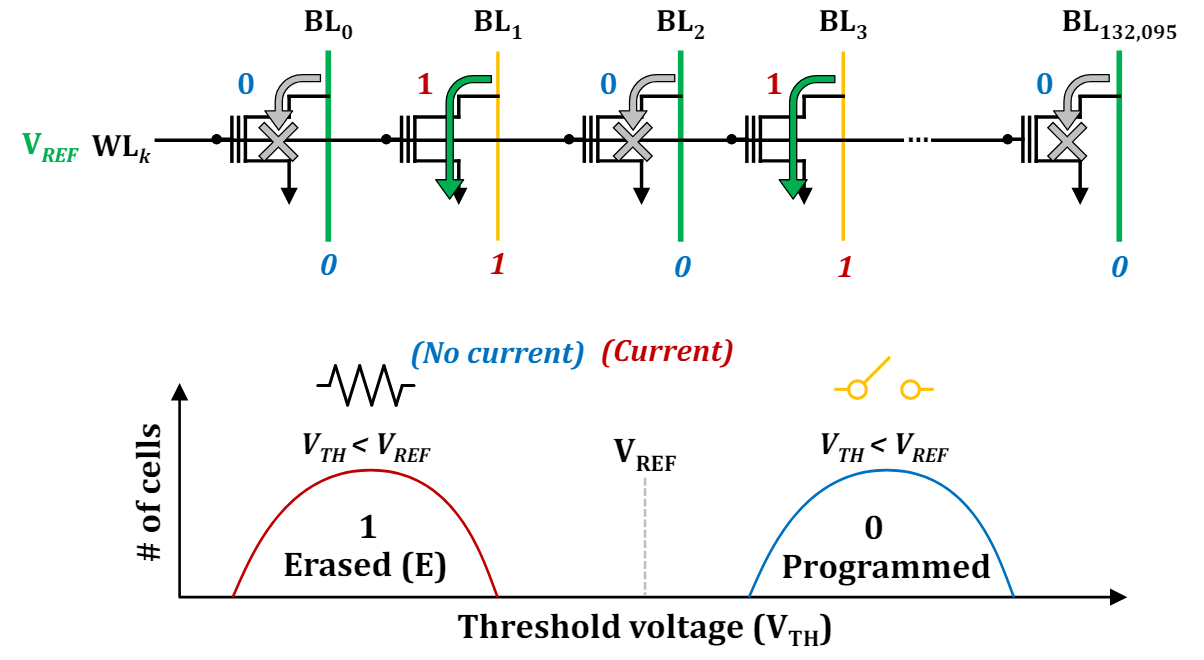
\includegraphics[width=0.6\linewidth]{img/amrytg.png}
\end{figure}


\section{Conclusioni}

Un SSD è un componente molto più complesso di quello che possa sembrare, monta un processore il quale deve tenere contro di varie problematiche quali:

\begin{itemize}
    \item l'usura deve essere uniforme,
    \item deve gestire dove scrivere i dati,
    \item quando eliminare un blocco,
    \item spostare qualche blocco,
    \item supervisione della salute dell'SSD, S.M.A.R.T.,
    \item ecc.
\end{itemize}

Una ram statica (cache) a confronto è molto più semplice.


